\chapter{The Gram-Schmidt process}
\label{sec:gs}

The Gram-Schmidt process takes a set of vectors and provides an orthonormal set of basis vectors. This process has two primary uses in the \svdp:
\begin{enumerate}
\item To build an orthonormal basis for a null space given a set of vectors in the image;
\item To orthonormalize the set of null space vectors output from a matrix reduction.
\end{enumerate}

%%
\section{Process schematic}
Start with a set of $k$ $\mv$s
\begin{equation}
  U = \lst{u_{1},u_{2},\dots,u_{m}}, \quad k\le m.
\end{equation}
If $j$ vectors are linearly independent, the Gram-Schmidt process will produce a set of $j$ orthonormal vectors
\begin{equation}
  V = \lst{\hat{v}_{1},\hat{v}_{2},\dots,\hat{v}_{j}}, \quad j\le k.
\end{equation}

A sample set input and output for two linearly independent vectors is shown in table \eqref{tab:gs:io}. The input set $U$ is shown on the left and the set $V$ is shown on the right. Part of the unit circle is included to show the effect of dilations upon the vectors. The Gram-Schmidt orthogonalization process is then displayed pictorially in the following table \eqref{tab:gs:guts}.

\begin{table}[htdp]
$$
\boxed{
\begin{array}{ccc}
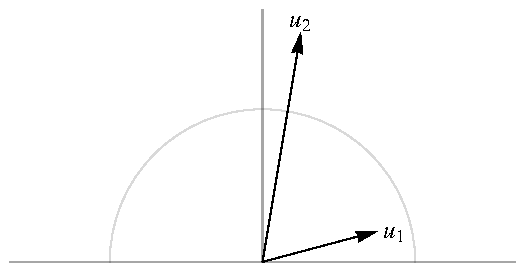
\includegraphics[ width = 2.25in ]{pdf/gs/gs_00.pdf} &
\Rightarrow &
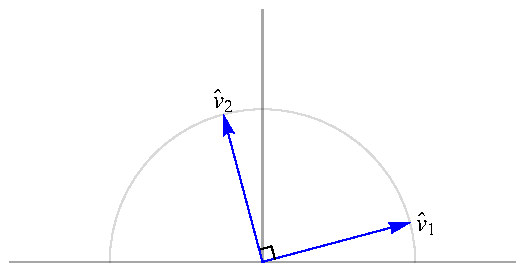
\includegraphics[ width = 2.25in ]{pdf/gs/gs_05.pdf}
\end{array}
}
$$
\label{tab:gs:io}
\caption[The Gram-Schmidt orthogonalization process]{The Gram-Schmidt orthogonalization process depicted for a set of two vectors. The input is the set of $u$ vectors on the left, the output are the orthonormal unit vectors $\hat{v}$ on the right. The vectors are plotted against the upper half of the unit circle to show the effect of dilations.}
\end{table}
%%%%
\begin{table}[top]
$$
\boxed{
\begin{array}{cc}
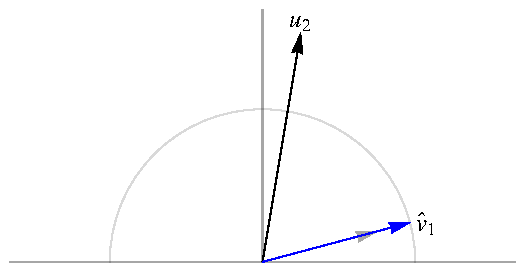
\includegraphics[ width = 2.25in ]{pdf/gs/gs_01.pdf} &
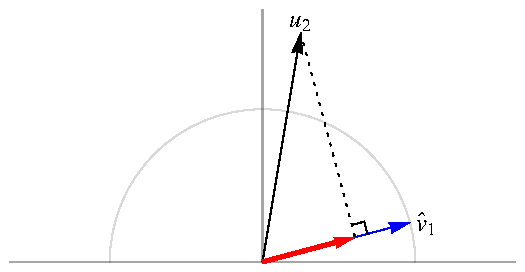
\includegraphics[ width = 2.25in ]{pdf/gs/gs_02.pdf} \\
\text{Step 1: normalization of $v_{1}$.} &
\text{Step 2: projection onto $v_{1}$.} \\[10pt]\hline
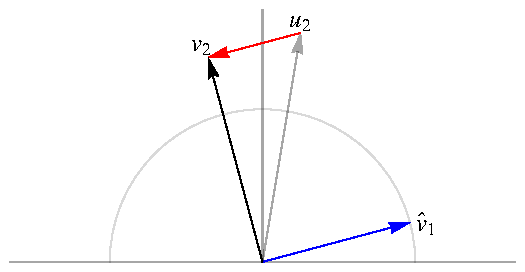
\includegraphics[ width = 2.25in ]{pdf/gs/gs_03.pdf} &
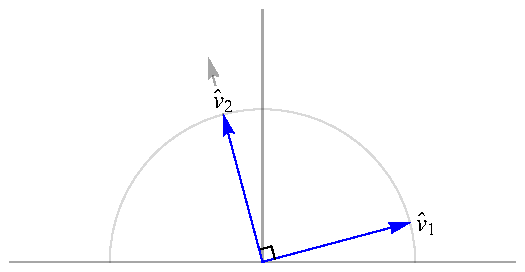
\includegraphics[ width = 2.25in ]{pdf/gs/gs_04.pdf} \\
\text{Step 3: subtract projection.} &
\text{Step 4: normalization of $v_{2}$.}
\end{array}
}
$$
\label{tab:gs:guts}
\caption[The Gram-Schmidt orthogonalization process for two vectors]{The Gram-Schmidt orthogonalization process is detailed for the two input vectors in the previous table. Pick an ordering to sweep through the set of vectors since the process is order dependent. The first action is to normalize the length of the first vector as shown in step 1. Find the orthogonal projection of the second vector onto the first vector. This projection is shown with the red arrow in step 2. For the next step, subtract this projection from the second vector which ``straightens up'' this vector as shown in step 3. Finally, normalize the new vector as shown in step 4.}
\end{table}

%%
\section{Projections}
The language of projections is a natural choice for a discussion of the Gram-Schmidt process as one may surmise from the previous table. Recall that the projection of a vector $y$ onto the vector $x$ is defined this way
\begin{equation}
  \pee{}_{x}(y) = \frac{y\cdot x}{x\cdot x}y.
\end{equation}
This notation allows for a compact and intuitive representation of the orthogonalization.

In two dimensions orthogonalization is simple. The generalization to higher dimensions looks follows here. Start with a list with a total of $m$ vectors $U$ in arbitrary ordering. The output will be a set of $n$ orthogonal vectors $V$ which depends upon the ordering of the vectors in the input set. The first few steps look like this:
\begin{equation}
  \begin{array}{cccccccccc}
    v_{1} &=& u_{1}\\
    v_{2} &=& u_{2} &-& \pee{}_{v_{1}}(u_{2})\\
    v_{3} &=& u_{3} &-& \pee{}_{v_{1}}(u_{3}) &-& \pee{}_{v_{2}}(u_{3})\\
    v_{4} &=& u_{4} &-& \pee{}_{v_{1}}(u_{4}) &-& \pee{}_{v_{2}}(u_{4}) &-& \pee{}_{v_{3}}(u_{4})\\
     & \vdots
  \end{array}
\end{equation}
The general formula takes the compact form
\begin{equation}
  \check{v}_{k} = u_{k} - \sum_{j}^{m-1}{\pee{}_{v_{j}}(u_{k})}
\end{equation}
where $\check{v}$ denotes an unnormalized vector.

If the vectors in the collection $U$ are linearly independent, then the collection $V$ will have the same number of vectors. That is, $m=n$. If the input vectors have linear dependencies then there will be fewer vectors in the output list and $m>n$. For this discussion only nonzero vectors are relevant.
 
At this juncture the vectors in the set $V$ are orthogonal, but not yet orthonormal. To normalize them use the prescription
\begin{equation}
  v_{k} = \frac{\check{v}_{k}}{\normt{\check{v}_{k}}}, \quad k=1,n.
\end{equation}

%%
\section{Application}
Let's return to a familiar example matrix to use the Gram-Schmidt orthogonalization process to compute a \svdl.

Consider the rank-deficient rectangular matrix
\begin{equation}
  \A{} = \Aexample.
\end{equation}

%%
\subsection{Column space: codomain}
As noted early and often, the column space contains one independent column vector
\begin{equation}
  c_{1} = \mat{r}{1\\-1\\1}.
\end{equation}
We need to stir in two other vectors. A good choice is to use two unit vectors. They are simple and it is easy to check that they are not linearly dependent upon the target vector $c_{1}$. The input vectors are these:
\begin{equation}
  U = \lst{u_{1},u_{2},u_{3}} = \lst{
  \mat{r}{1\\-1\\1},
  \mat{r}{1\\0\\0},
  \mat{r}{0\\1\\0}
  }.
\end{equation}

%%
\subsubsection{First vector}
The first vector is the easiest. It requires a scaling, or dilation, to normalize the length:
\begin{equation}
  v_{1} = \frac{u_{1}}{\normt{u_{1}}} = \sthree
  \mat{r}{1\\-1\\1}.
\end{equation}

This action corresponds to step 1 in table \eqref{tab:gs:guts} above.

%%
\subsubsection{Second vector}
The first part of this step is to compute the projection of the input vector $u_{2}$ onto the previous output vector $v_{1}$:
\begin{equation}
  \pee{}_{v_{1}}(u_{2}) = \rthree\mat{r}{1\\-1\\1}.
\end{equation}
This projection corresponds to the red vector in step 2 in table \eqref{tab:gs:guts}.

The unnormalized output vector becomes this
\begin{equation}
  \check{v}_{2}= u_{2} - \pee{}_{v_{1}}(u_{2}) = \rthree \mat{r}{2\\1\\-1}.
\end{equation}
This corresponds step 3 in table \eqref{tab:gs:guts}.

The normalized form is then
\begin{equation}
  v_{2} = \ssix \mat{r}{2\\1\\-1}.
\end{equation}
This is the final step, the fourth step in table \eqref{tab:gs:guts}.

%%
\subsubsection{Third and final vector}
We need to project the final input vector $u_{3}$ onto the subordinate output vectors. The projections are these
\begin{equation}
  \begin{split}
    \pee{}_{v_{1}}(u_{3}) = \rthree \mat{r}{-1\\1\\-1}, \quad \pee{}_{v_{2}}(u_{3}) &= \rsix   \mat{r}{1\\1\\-1}.
  \end{split}
\end{equation}

The unnormalized output vector becomes this
\begin{equation}
  \check{v}_{2}= u_{3} - \pee{}_{v_{1}}(u_{3}) - \pee{}_{v_{2}}(u_{3}) = \rtwo \mat{r}{0\\1\\1}.
\end{equation}

The final normalized form is given by this
\begin{equation}
  v_{2} = \stwo \mat{r}{0\\1\\1}.
\end{equation}

%%
\subsubsection{Assemble the codomain matrix}
The result from the Gram-Schmidt procedure are these three orthonormal vectors:
\begin{equation}
  V = \lst{v_{1},v_{2},v_{3}} = \lst{
  \sthree \mat{r}{1\\-1\\1},
  \ssix   \mat{r}{2\\1\\-1},
  \stwo   \mat{r}{0\\1\\1}
  }.
\end{equation}
These vectors are the column vectors of the codomain matrix:
\begin{equation}
  \Y{} = \mat{c|c|c}{v_{1} & v_{2} & v_{3}} =
\left[
\begin{array}{ r >{\columncolor{ltgray}}r >{\columncolor{ltgray}}c }
  \sthree &  \frac{2}{ \sqrt{6} } & 0  \\[5pt]
 -\sthree &  \ssix & \stwo \\[5pt]
  \sthree & -\ssix & \stwo 
\end{array}
\right] 
\end{equation}

%%
\subsubsection{Check the final answer}
A quick, easy and helpful check involves verifying the orthogonality of the vectors $V$:
\begin{equation}
  \begin{split}
    v_{1}\cdot v_{2} &= 0,\\
    v_{1}\cdot v_{3} &= 0,\\
    v_{2}\cdot v_{3} &= 0.\\
  \end{split}
\end{equation}

%%
\subsection{Row space: domain}
\label{sec:gs:row}
The row space here too contains one independent vector
\begin{equation}
  r_{1} = \mat{r}{1\\-1}.
\end{equation}
This time we need only one candidate \vv \ to complete the space. The two input vectors are these:
\begin{equation}
  U = \lst{u_{1},u_{2}} = \lst{
  \mat{r}{1\\-1},
  \mat{r}{1\\0}
  }.
\end{equation}

%%
\subsubsection{First vector}
The first vector only requires normalization:
\begin{equation}
  v_{1} = \frac{u_{1}}{\normt{u_{1}}} = \stwo
  \mat{r}{1\\-1}.
\end{equation}

Notice that $v_{1}\cdot v_{2}=0$.

%%
\subsubsection{Second and final vector}
The projection of the second input vector $u_{2}$ onto the first output vector $v_{1}$:
\begin{equation}
  \pee{}_{v_{1}}(u_{2}) = \rtwo\mat{r}{1\\-1};
\end{equation}
this leads to the unnormalized output vector:
\begin{equation}
  \check{v}_{2}= u_{2} - \pee{}_{v_{1}}(u_{2}) = \rtwo\mat{r}{1\\1};
\end{equation}
with the normalized form given here
\begin{equation}
  v_{2} = \stwo \mat{r}{1\\1}.
  \label{eq:gs:a}
\end{equation}

%%
\subsubsection{Assemble the domain matrix}
The column vectors of the domain matrix are these output vectors
\begin{equation}
  \X{} = \mat{c|c}{v_{1} & v_{2}} = \Xshade.
\end{equation}

%%
\subsection{Assemble the SVD}
Given the domain matrices $\X{}$ and $\Y{}$, the only remaining piece is the singular values. Since the target matrix had only one independent column\footnote{One could also base the rank argument on the number of independent rows.} the rank is $\rho = 1$. The $\sig{}$ matrix always has the same shape as the target matrix. Therefore we are solving for this matrix:
\begin{equation}
  \sig{} = \mat{c|c}{\sigma_{1} & 0 \\\hline 0 & 0 \\ 0 & 0}.
\end{equation}
We can glean the lone singular value $\sigma_{1}$ from this equation:
\begin{equation}
  \begin{split}
    \A{}\X{}_{*,1} &= \sigma_{1}\Y{}_{*,1},\\
    \Aexample \stwo \mat{r}{1\\-1} &= \sigma_{1} \sthree \mat{r}{1\\-1\\1}.
  \end{split}
\end{equation}
This leads to the reassuring conclusion that
\begin{equation}
  \sigma_{1} = 6^{-1/2}.
\end{equation}

Compare the top SVD from the Gram-Schmidt process to the bottom form computed in \eqref{eq:simple:svd}
\begin{equation}
  \begin{array}{rcccc}
    \A{} &=& \Y{} & \sig{} & \X{T} \\
      &=& \left[
\begin{array}{ r >{\columncolor{ltgray}}r >{\columncolor{ltgray}}c }
  \sthree &  \frac{2}{ \sqrt{6} } & 0  \\[5pt]
 -\sthree &  \ssix & \stwo \\[5pt]
  \sthree & -\ssix & \stwo 
\end{array}
\right]  
   & \Sigmaexampleb 
   & \Xtshade;\\[15pt]
   &=& \Yshade & \Sigmaexampleb & \Xtshade.
  \end{array}
\end{equation}

Two different processes yielded different yet equivalent \svdl s. The $\sig{}$ matrices must be the same. The domain matrices may have some sign difference in the range vectors. In this case the range vectors, the unshaded vectors in the $\X{}$ and $\Y{}$ matrices match for both decomposition methods. The null space (shaded) vectors in the codomain matrix $\Y{}$ are ordered differently. Also, there are sign differences between the shaded column vectors.

%%
\subsection{Superfluous vectors}
Let's explore the case where the vector collection $U$ has two many vectors. For example, suppose $U$ has three \vv s. The output collection $V$ will only have two orthogonal unit \vv s. How does a vector dissappear?

Go back to \S\eqref{sec:gs:row} and append a vector to the input collection:
\begin{equation}
  U = \lst{
  \mat{r}{1\\-1},
  \mat{r}{1\\0}
  }
  \quad \rightarrow \quad
  \lst{
  \mat{r}{1\\-1},
  \mat{r}{1\\0},
  \mat{r}{0\\1}
  }.
\end{equation}

We can pick up the calculation for $\check{v}_{3}$ after equation \eqref{eq:gs:a}:
\begin{equation}
  \begin{split}
    \check{v}_{3} &= u_{3} - \pee{}_{v_{1}}(u_{3}) - \pee{}_{v_{2}}(u_{3})\\
    & = \mat{c}{0\\1} - \rtwo\mat{r}{-1\\1} - \rtwo\mat{c}{1\\1}\\
    & = \mat{r}{0\\0}.
  \end{split}
\end{equation}
The first two output vectors, $v_{1}$ and $v_{2}$, completely span the space $\real{2}$. No other vectors are needed and the Gram-Schmidt process will produce zero vectors after this iteration.

Further readings: \cite[ch. 5.5, p. 307]{Meyer}[ch. 5.5, p. 307]{}, Strang[]{}.


\endinput